\subsection{Kiểm thử các thành phần Frontend}

Kiểm thử Frontend tập trung vào việc đảm bảo tính đúng đắn của logic giao diện, tính tương tác của các component và sự ổn định của luồng nghiệp vụ trên trình duyệt.

\subsubsection{Chiến lược kiểm thử tự động (Automated Testing)}

Nhóm áp dụng khung làm việc \textbf{Vitest} kết hợp với \textbf{React Testing Library (RTL)} để thực hiện kiểm thử đơn vị và kiểm thử thành phần. Vitest được lựa chọn vì tốc độ thực thi cực nhanh và khả năng tương thích hoàn hảo với hệ sinh thái Vite/Next.js.

\textbf{Mô hình kiểm thử dựa trên hành vi người dùng}

Thay vì kiểm tra trạng thái nội bộ của component, nhóm tập trung vào kiểm tra cách người dùng tương tác với giao diện. Chiến lược này giúp các bài test bền bỉ hơn khi cấu trúc code thay đổi. Quy trình thực hiện cũng tuân thủ mô hình \textbf{AAA (Arrange -- Act -- Assert)}:
\begin{itemize}
    \item \textbf{Arrange:} Khởi tạo component trong môi trường giả lập (jsdom), cung cấp các mock data và thiết lập các provider (Theme, Auth, Query Client).
    \item \textbf{Act:} Giả lập các hành động của người dùng như nhấn nút, nhập liệu vào form bằng thư viện \texttt{@testing-library/user-event}.
    \item \textbf{Assert:} Khẳng định sự thay đổi trên giao diện (ví dụ: thông báo thành công hiện lên, dữ liệu mới được hiển thị) thông qua các câu lệnh \texttt{expect}.
\end{itemize}

\textbf{Mocking và Isolation}

Để cô lập các bài test khỏi sự phụ thuộc vào Backend thực tế, nhóm sử dụng kỹ thuật Mocking cho các module gọi API. Các phản hồi từ server được giả lập để kiểm tra các trường hợp khác nhau như: dữ liệu trả về thành công, lỗi server (500), hoặc lỗi không tìm thấy (404).

\subsubsection{Kiểm thử thủ công và Trải nghiệm người dùng (Manual & UX Testing)}

Bên cạnh kiểm thử tự động, nhóm thực hiện các đợt kiểm thử thủ công để đánh giá các khía cạnh mà máy tính chưa thể kiểm tra hoàn hảo:
\begin{itemize}
    \item \textbf{Kiểm thử giao diện phản hồi (Responsive Testing):} Kiểm tra khả năng hiển thị và tương tác trên nhiều kích thước màn hình khác nhau (Mobile, Tablet, Desktop).
    \item \textbf{Kiểm thử luồng hội thoại AI:} Tương tác trực tiếp với Trợ lý Ảo để đánh giá tính hợp lý của các câu trả lời, tốc độ phản hồi streaming và khả năng xử lý các yêu cầu phức tạp từ khách hàng.
    \item \textbf{Kiểm thử khả năng truy cập (Accessibility Testing):} Sử dụng các công cụ như Lighthouse để đảm bảo giao diện thân thiện với mọi đối tượng người dùng.
\end{itemize}

\subsubsection{Thống kê kết quả kiểm thử Frontend}

Dưới đây là bảng thống kê tóm tắt kết quả kiểm thử cho các thành phần Frontend:

\begin{table}[H]
\centering
\small
\begin{tabular}{|c|l|l|c|c|c|}
\hline
\textbf{STT} & \textbf{Module} & \textbf{Thành phần kiểm thử} & \textbf{Pass} & \textbf{Fail} & \textbf{Tổng} \\ \hline
1 & Auth & Logic Đăng nhập, Đăng ký, Quên mật khẩu & 45 & 0 & 45 \\ \hline
2 & Product & Hiển thị danh sách, Bộ lọc, Chi tiết sản phẩm & 65 & 0 & 65 \\ \hline
3 & Cart & Thêm/Xóa sản phẩm, Cập nhật số lượng & 40 & 0 & 40 \\ \hline
4 & Order & Luồng thanh toán, Theo dõi đơn hàng & 35 & 0 & 35 \\ \hline
5 & AI Chatbot & Gửi nhận tin nhắn, Hiển thị card sản phẩm & 25 & 0 & 25 \\ \hline
6 & Common UI & Các component dùng chung (Button, Input, Modal) & 76 & 0 & 76 \\ \hline
\multicolumn{3}{|c|}{\textbf{TỔNG CỘNG FRONTEND}} & \textbf{286} & \textbf{0} & \textbf{286} \\ \hline
\end{tabular}
\caption{Thống kê kết quả kiểm thử tự động tầng Frontend}
\label{tab:frontend_test_summary}
\end{table}
\vfill
\begin{figure}[H]
    \centering
    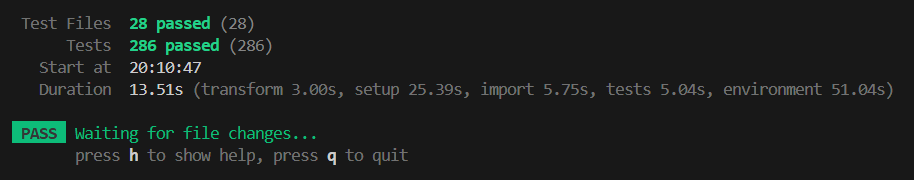
\includegraphics[width=0.8\textwidth]{images/chap8/testing/vitest_summary.png}
    \caption{Kết quả thực thi 286 test cases bằng Vitest}
    \label{fig:vitest_results}
\end{figure}

\begin{figure}[H]
    \centering
    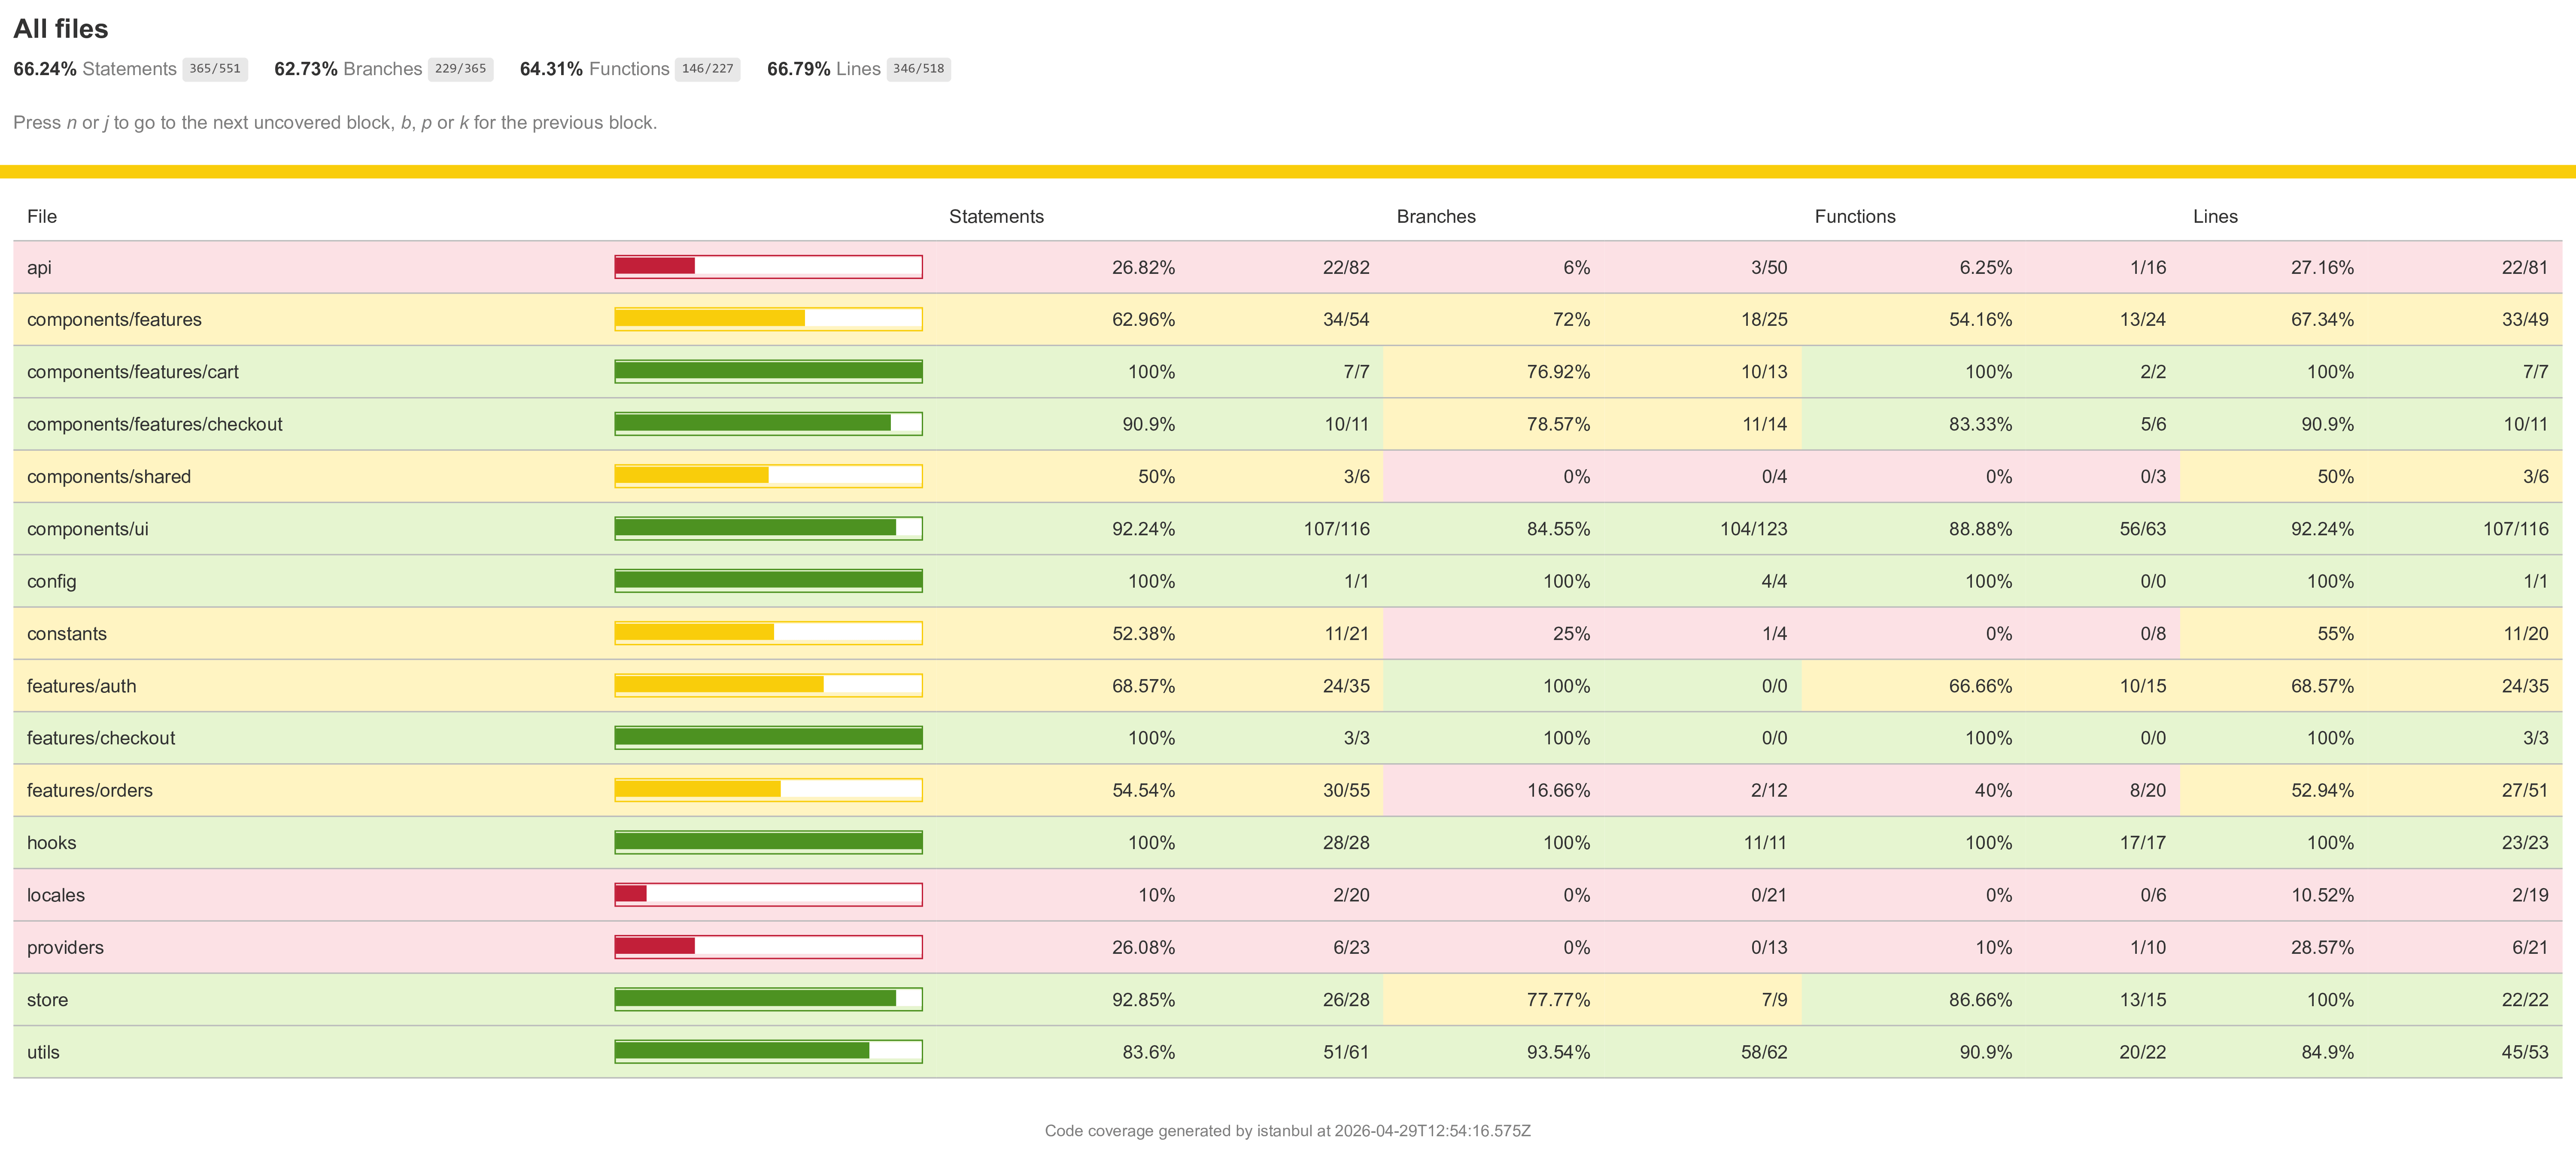
\includegraphics[width=0.9\textwidth]{images/chap8/testing/coverage_dashboard.png}
    \caption{Báo cáo độ bao phủ mã nguồn (Code Coverage) chi tiết của tầng Frontend}
    \label{fig:coverage_report}
\end{figure}
